In recent decades, cognitive science has deepened our understanding of the mechanisms that subserve skill learning and has begun to spark ideas on how to achieve better learning by leveraging these mechanisms more effectively. Thus far, most studies have focused on simple, laboratory-based tasks, raising concerns about their applicability to real-world learning in areas such as sports, education, or rehabilitation. Therefore, there is a pressing need for studies with greater ecological validity, where learning tasks are not trivial exercises but instead improve important life functions or skills that learners genuinely care about. The overarching goal of this doctoral thesis was to bridge this gap between simple tasks and real-world skill learning with skilled performers using alpine skiing as a domain to test these theories. To achieve this goal, this doctoral thesis adopted a crossdisciplinary research approach involving mechanics and psychology. From a mechanical perspective, we asked what is the most effective strategies for skiing faster on flat slopes (aim 1) and the kinematic signatures that make one of these strategies so effective (aim 2). From a psychological perspective, we asked whether better learning effects could be achieved by applying learning theories from cognitive science to create learning problems (aim 3) and better utilize teaching signals (aim 4).  

First, we found that skiers on average achieved the fastest race times using the "extend with rock skis forward" strategy, which aligns with our expectations based on theory and quantitative field observations. This suggests that this strategy is powerful and can improve the performance of skiers on flats in slalom. However, its effect was only marginally better than that of the "extend" strategy, which is simpler and nearly as effective on its own. Based on these results, we recommend that skiers choose either of these two strategies to enhance their performance on flat sections in slalom. These findings expand upon previous ski research and provide experimental evidence for effective strategies to ski fast on flats in slalom.

Second, we also found that a training intervention focusing on the "extend" strategy left a remarkable kinematic signature on the skiers. After the intervention, skiers exhibited a more wave-like speed profile. That is, they increased their speed after passing through a gate, which continued to rise until they were approximately midway between two gates. Then, their speed decreased until the next gate, before increasing again. Additionally, we observed a trend where skiers took longer paths between gates, yet their race times improved. Together, these kinematic signatures closely resemble the predictions from Lind and Sander's model of pumping to increase velocity. A limitation of our data is that we do not know the specific movements the skiers made, preventing us from testing the model's predictions accurately. Future research should employ motion capture technology to achieve the necessary data quality for such investigations.

Shifting focus toward the testing of learning theories to improve skill learning, we did not find evidence that the skiers learned better by increasing the frequency at which they were exposed to new learning problems (that is, interleaved practice). This finding aligns with prior research that has similarly failed to observe a contextual interference effect in real-world tasks or more complex learning tasks \cite{brady_theoretical_1998, barreiros_contextual_2007, wulf_principles_2002}. Based on the results of this study and these previous findings, it may not be worthwhile to expend effort in creating multiple different slalom courses, at least concerning performance outcomes. Nonetheless, we should not dismiss the possibility that exposing skiers to rapid changes in course could influence other cognitive mechanisms. It is also plausible that the benefit of frequent course changes lies in preventing habits \cite{du_relationship_2022}, whereby skiers settle on a fixed solution and become insensitive to adapting to different situations. If so, simply changing courses sufficiently often might be adequate to avoid these habits. To better understand this phenomenon, an alternative experimental design is crucial. One approach could involve training hairpin, with one learning group practising only one hairpin while another group practising multiple hairpins.

Til slutt vi fant at å lære strategier 
 














Vi fant også en treningsintervensjon på "extend" strategien etterlot seg en interessant kinematisk signatur på utøveres skikjøring. Etter intervensjonen fant vi at utøverne sin fartsprofil var betydelig mer bølgeformede, der skiers increased their speed after gate passage which continued to rise until they were approximately midway between two gates. After that, the speed decreased to the gate before it rose again. I tillegg fant vi en trend til at utøverne kjørte en lenger path length mellom gates, men til tross for at renntidene ble bedre. Den kinematiske signaturen minner dermed veldig om prediksjonene fra Lind and Sander's modell på pumping. I begrensning med disse dataene er at vi ikke vet hvilke bevegelser utøverne faktisk gjorde, og vi har dermed i mulighet for å teste prediksjonene fra modellen. Fremtidig forskning bør gjøre nærmere undersøkelser med motion capture for å oppnå denne nødvendige datakvalitaten.















Forflytter oss bort fra strategienes effekter og til testing læringsteoriene, fant vi ingen statistisk signifikant learning effekt av contextual interference to increase the frequency at which skiers are exposed to new learning problems. This finding aligns with previous research that has not found a contextual interference effect in real-world tasks or more complex activities \cite{brady_theoretical_1998, barreiros_contextual_2007, wulf_principles_2002}. Basert på resultatene fra denne og disse tidligere studiene er det ikke verdt effort å sette mange forskjellige slalomløyper iallefall når det kommer til prestasjon. Vi skal likevel ikke utelukke at å exponere utøvere for rapid bytter av løyper kan exert influence på andre kognitive mekanismer som motivasjon og som vi ikke har målt i denne studien. Det kan også være at gevinsten av å bytte løyper ofte er at man skal unngå habits, som at utøvere finner en løsning og blir insensitiv til å endre løsning til andre situasjoner. I så fall kan det muligens være nok å bytte løyper tilstrekkelig ofte slik at man unngår disse habitene. For å bedre forstå dette er det viktig med et annet eksperimentelt design. En måte å gjøre dette på er å trene hårnåler der en læringsgruppe kun trener en hårnål, mens en annen gruppe trener flere hårnåler. 















Our data indicate that the intervention increased the speed and path length in certain gate sections. How does this align with previous alpine research and mechanical theories on pumping? First, these and previous results suggest that the pumping ("extend") strategy might exert a real impact on skiers' speed and performance in flat sections, contrary to previous beliefs \cite{supej_differential_2008, supej_doba_2001}. The increased speed from turn to turn and the distinct change in the speed profile align well with expectations from a pumping mechanism to increase the speed from turn to turn. It therefore appears that skiers can pump themselves to higher speeds and that this is an important mechanism to leverage in align with Lind and Sander's model \cite{lind_physics_2004}. We also observed a trend where the path length increased slightly from gate to gate, although this varied significantly from turn to turn. Several factors could explain this increased path length, which we cannot quantify or separate using the local positioning system. One possibility is that pumping increases the path length because the extension movement exerts more force on the skis, causing them to bend and turn more. However, this could also result from measurement errors from the local positioning systems or differences in the course setting.

























og denne studien er den første som gir eksperimentell evidens for at utøvere 


men strategien var riktignok kun marginalt bedre enn å strekke alene. Det ser dermed ut til at å strekke i seg selv var en powerful strategi. Utøvere bør derfor bruke ekstend eller extend with rock skis forward når de kjører flater. Når imidlertid helningsvinkelen øker og det blir vanskeligere å bruke disse strategiene bør utøvere bytte strategi. Den utfordrende oppgaven er å finne ut når man kan bruke ekstend og når man skal bruke andre strategier. Dette er interessant å studere i videre forskning.

For det andre så vi at


Vi fant også at reinforcement learning var et effektivt teaching signal som kan brukes for å trene gode athletes. 















our research strategy was to develop knowledge about the skills and strategies that 


these skilled performers use to enhance their performance further and actively use this knowledge to create interventions for relevant skills to test these learning theories. This dissertation had two main objectives: first, to identify the most effective strategies for high-speed performance on flat surfaces and to understand why these strategies are effective; second, to determine whether cognitive science learning strategies can improve learning situations for performers through more effective problem-solving methods and the use of effective teaching signals. 






In recent decades, cognitive science has accentuated our understanding of the mechanisms that likely exert control of skill learning, og øynet håp om hvordan de kan utnyttes bedre for mer effektive læring. However, most of these studies have been performed with simple, laboratory-based tasks, raising concerns about their generalizability to real-world learning, such as sports, education, or rehabilitation. Therefore, there is a pressing need for studies with greater ecological validity, where the learning task not is a trivial exercise but may improve important life functions or skills that learners genuinely care about. Det overordnede målet med denne doktorgraden var derfor å bridge dette gapet mellom enkle oppgaver og komplekse real world skills med gode utøvere. Den valgte forskningtilnærmingen for å få til denne bridgingen var å bygge opp kunnskap om ferdigheter og strategier som disse gode utøverne kan bruke for å løfte prestasjonen videre, og deretter aktivt bruke denne kunnskapen til å lage intervensjoner på relevante ferdigheter for å teste disse læringsteoriene. Doktorgraden har således hatt to hovedmål: for det ene var det å finne ut hvilke strategier som er mest effektive for å kjøre raskt på flater og å forstå hvorfor disse strategiene er effektive. For det andre var det å forstå om disse læringsstrategiene fra kognitive vitenskap kan brukes til å forbedre læringssituasjoner hos utøvere gjennom mer effektive måter å lage læringsproblemer på og bruk av effektive teaching signals.

Det første spørsmålet som ble addressert i denne doktorgradenvar om 



Cognitive science has made great strides in understanding the mechanisms that likely exert control of skill learning and how they can be leveraged to improve learning and performance \cite{wolpert_principles_2011, makino_circuit_2016, spampinato_multiple_2021, krakauer_motor_2019, haith_model-based_2013, huang_rethinking_2011, shmuelof_are_2011, doya_complementary_2000}. 






\subsubsection{Quantifying performance in alpine skiing}
One of the key objectives of this doctoral project was to determine a reliable method for quantifying performance in alpine skiing over time, whether over days, weeks, or months. One of the greatest challenges in this respect, from a scientific perspective, is its lack of standardization; the time taken to ski a slalom course one day may not be comparable to that of another day  Consequently, quantifying performance in alpine skiing has been widely debated, with scientists arguing for measures such as energy mechanics \cite{supej_differential_2008, supej_how_2010, supej_mechanical_2011} , differences in mechanical energy divided by time, section times \cite{supej_relations_2006}, lateral skidding of skis \cite{kirby_development_2009}, and time loss per elevation difference and distance travelled per elevation difference \cite{federolf_quantifying_2012}. Throughout my doctoral research, I have chosen to express performance in terms of time, which is the conventional way to quantify performance in skiing and allowed me to operate on the same scale as skiers and coaches do. In my doctoral reseach, I have adopted two different time measures: in papers 1 and 2, I have expressed time as the difference from the time when the skier skied the section straight down (straight gliding), whereas, in paper 3, I used the raw time to quantify performance. Here, I aim to provide some methodological reflections on these approaches to help readers evaluate the results of the studies in this doctoral thesis and to assist other researchers in the field of alpine skiing. 

To begin this methodological consideration, I conducted a Bayesian multilevel growth model on all the skiers' times as they skied straight down the section for all sessions in paper 3. From this analysis, I found that the straight gliding times for all ski groups (A, B, C, and D) increased steadily from the first session (baseline) to the last session (transfer). Although I cannot rule out any explanation for why the straight gliding times of the ski groups increased uniformly, I am confident that differences in the length of the course section are not the main explanation. This is because we used a measuring tape during the course setting, and there was a tight cluster of boreholes at the finish line, with only a few centimeters of difference. I also do not believe that changes in the skiers' starting procedures or execution of straight gliding are the main reasons. This is because the skiers were diligent and interested in performing this task as well as possible. I believe the best explanation involves the snow conditions and how we prepared them. Specifically, when grooming snow with a machine, grooves are left in the snow that becomes hard if it is watered and allowed to freeze. These hard grooves are fast to ski on because only a small part of the ski is in contact with the snow surface. As skiers complete more runs and coaches slide through the course, these snow grooves wear away, creating a smooth, hard base without grooves. When skiers descend on this groom-free base, a larger part of the ski’s contact surface touches the snow, which increases ski–snow friction and slows the skiers down.

The question is, what consequences does this have for the results, and how can we address these challenges the best possible way? First, one challenge this creates is the need to exercise caution in interpreting 'true' learning from the estimated change in race times. From From Fig. \ref{fig:rlstudy_racetime} from Study \RNum{2}, we find that the skiers improved their race times significantly over the sessions despite the increased straight gliding times. Therefore, the 'true' improvement is likely better than estimated. A less conservative and perhaps better way to express skiers' 'true' learning is to use the difference in straight gliding times for each session to account for variations in the snow surface. This is the performance measure we used in Study\RNum{1}. However, although this measure may better capture skiers' learning, we do not know whether it underestimates or overestimates learning. Another problem is that straight gliding in itself is a random variable that introduces variation and could add noise to the measurement. In Study \RNum{2}, we had to move away from this measure because the straight gliding lane crossed many holes from the previous courses. Due to these challenges, it is difficult to determine the actual improvement of skiers. Scientists therefore face two choices: either use raw race times, which is likely a conservative method that underestimates the real improvement, or express time as the difference in straight gliding, which may better account for variations in the surface and therefore express progress more accurately. The cost of the latter approach is that it underestimates or overestimates performance and could increase noise. 

Another solution is to downplay the focus on change and determine whether the learning groups differ on the postmeasure if their performance is equal at baseline, corresponding to the logic of an ANCOVA. If we have a design where skiers have undeone tests simultaneously, we can estimate this group difference, indirectly avoiding the question of change. Therefore, we used ANCOVA and raw race data in Study \RNum{2}.

One potential way to improve estimates in future research is to test more levels within the ski groups. This would allow the groups to have varying effects of the treatment and achieve better estimates through partial pooling \cite{mcelreath_statistical_2018}. We attempted to run this model, but it did not converge due to having too few levels. It might have been better to divide the ski groups into smaller subgroups that were tested at different times. This approach could have provided more levels and potentially better estimates through partial pooling. However, it must be emphasized that conducting studies such as ours is very difficult and time-consuming. Another approach is to skid extensively to eliminate the grooms before testing. 


\begin{figure}
    \centering
    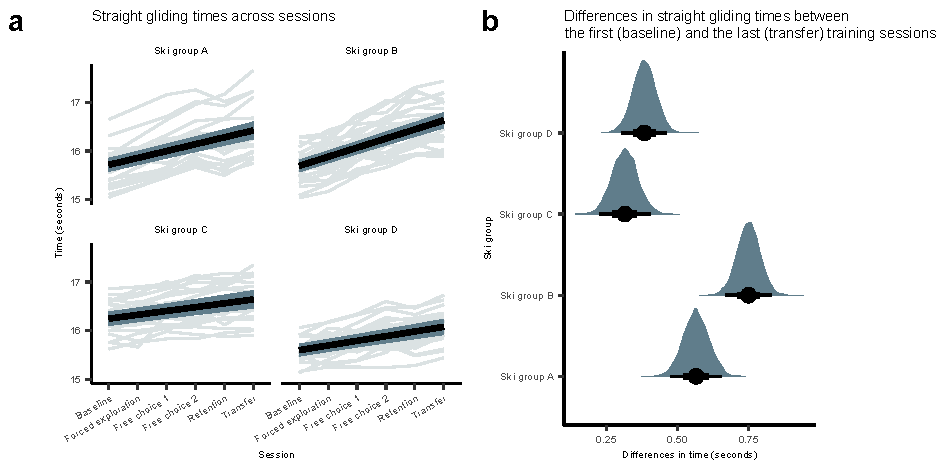
\includegraphics[width=1\linewidth]{figure/figure_methodological_straightgliding.pdf}
    \caption{Enter Caption}
    \label{fig:straightgliding}
\end{figure}